\documentclass{article}
\usepackage{amsmath}
\usepackage{titlesec}
\usepackage{graphicx}
\usepackage[margin=1in]{geometry}
\usepackage{hyperref}

% Title, date, and author
\title{Project 1}
\author{Your Name, Collaborator's Name}
\date{\today}

\titleformat{\section}
  {\normalfont\normalsize\bfseries} % Format: font style, size, and weight
  {\thesection}{1em} % Label format and spacing
  {}
  \renewcommand{\thesubsection}{\thesection.\alph{subsection}}

\titleformat{\subsection}
  {\normalfont\small\bfseries} % Format: font style, size, and weight
  {\thesubsection}{1em} % Label format and spacing
  {}
\titleformat{\subsubsection}
  {\normalfont\small\bfseries} % Format: font style, size, and weight
  {\thesubsubsection}{1em} % Label format and spacing
  {}

\begin{document}
\begin{titlepage}
    \centering
    \vspace*{1in}
    
    {\Huge\bfseries Project 1\par}
    \vspace{1.5cm}
    {\Large \today\par}
    \vspace{1.5cm}
    {\Large\itshape Antonio Pampalone 23586519 \\ Giuseppe Pisante 23610012\\ Martina Raffaelli 23616907 \par}
    
    \vfill
    
\includegraphics[width=0.3\textwidth]{FAU-Logo.png}\par\vspace{1cm} % Adjust the width as needed
   
\end{titlepage}

\newpage
\small

\section*{\Large Task 1.0:}

The boundary conditions are consistent with each other because they impose a continuous solution at the boundaries, and they set identical values at the points where they meet. However, the initial conditions are not consistent with the boundary conditions, since they impose different values on the edges of the domain than those specified by the boundary conditions. Because of the non consistency, we consider the initial conditions to be applied only on the inner part of the domain: $\Omega \setminus \partial \Omega$. 

\section*{\Large Task 1.1:}

\subsection*{Discretization with central differencing scheme in space and Crank-Nicolson method in time:}

Starting from the equation reported below, we first discretize the left-hand side term using Crank-Nicolson (C-N) method in time and then we discretize the right-hand side term following the central differencing scheme (CDS).
\begin{equation} 
  \frac{\partial T}{\partial t} = \frac{\partial^2 T}{\partial x^2} + \frac{\partial^2 T}{\partial y^2} \label{eq_reference}
\end{equation}
By applying C-N method to the time derivative we get the approximation:
\begin{equation} 
  \frac{\partial T}{\partial t} \approx \left(\frac{\partial T}{\partial t}\right)_{i,j} = \frac{T_{i,j}^{n+1} - T_{i,j}^n}{\Delta t} = \frac{1}{2}\left(\left(\frac{\partial^2 T}{\partial x^2} + \frac{\partial^2 T}{\partial y^2}\right)^{n} + \left(\frac{\partial^2 T}{\partial x^2} + \frac{\partial^2 T}{\partial y^2}\right)^{n+1}\right) \label{time_discretization}
\end{equation}
By applying CDS to both the spatial derivatives we get the approximations:
\begin{equation} 
  \frac{\partial^2 T}{\partial x^2} \approx \left(\frac{\partial^2 T}{\partial x^2}\right)_{i,j} = \frac{T_{i+1,j} - 2T_{i,j} + T_{i-1,j}}{(\Delta x)^2}, \label{space_discretization}
  \frac{\partial^2 T}{\partial y^2} \approx \left(\frac{\partial^2 T}{\partial y^2}\right)_{i,j} = \frac{T_{i,j+1} - 2T_{i,j} + T_{i,j-1}}{(\Delta y)^2}
\end{equation}

Now we substitute \eqref{space_discretization} into \eqref{time_discretization} as follows:
\begin{multline}
  \frac{T_{i,j}^{n+1} - T_{i,j}^n}{\Delta t} = \frac{1}{2}\left(\frac{T_{i+1,j}^n - 2T_{i,j}^n + T_{i-1,j}^n}{\Delta x^2} \right.\\
  + \frac{T_{i,j+1}^n - 2T_{i,j}^n + T_{i,j-1}^n}{\Delta y^2} +\frac{T_{i+1,j}^{n+1} - 2T_{i,j}^{n+1}+ T_{i-1,j}^{n+1}}{\Delta x^2} \\
  \left. + \frac{T_{i,j+1}^{n+1} - 2T_{i,j}^{n+1} + T_{i,j-1}^{n+1}}{\Delta y^2}\right)
\end{multline}
and we finally get:
\begin{multline} \label{final_discretization}
  T_{i,j}^{n+1} = T_{i,j}^n + \frac{\Delta t}{2}\left(\frac{T_{i+1,j}^n - 2T_{i,j}^n + T_{i-1,j}^n}{\Delta x^2} \right. \\
  + \frac{T_{i,j+1}^n - 2T_{i,j}^n + T_{i,j-1}^n}{\Delta y^2} + \frac{T_{i+1,j}^{n+1} - 2T_{i,j}^{n+1} + T_{i-1,j}^{n+1}}{\Delta x^2}\\
  \left.+ \frac{T_{i,j+1}^{n+1} - 2T_{i,j}^{n+1} + T_{i,j-1}^{n+1}}{\Delta y^2}\right)
\end{multline}

\subsection*{Stability of Crank-Nicolson method:}

The Crank–Nicolson method is a numerically stable method that is unconditionally stable for diffusion equations, meaning that its stability does not depend on the time step size $\Delta t $. However, the method may have an oscillatory behavior when using large time steps, high initial gradients, or in cases with transport-dominated problems. These oscillations are a characteristic behavior of the method for certain problem types, not a sign of instability.

\subsection*{Truncation error of Crank-Nicolson method:}

To compute the truncation error for the Crank–Nicolson method, we need to compare the continuous time derivative with the discrete approximation provided by the method.

The Crank–Nicolson scheme updates the solution \( T_{i,j} \) in time as follows:
\begin{equation}
T_{i,j}^{n+1} = T_{i,j}^n + \frac{\Delta t}{2} \left( f(T_{i,j}^{n+1}) + f(T_{i,j}^n) \right),
\end{equation}

To analyze the truncation error, we compare this discrete form to the exact time derivative using Taylor series expansion around \( T(t) \) reported below

\begin{equation*}
T(t + \Delta t) = T(t) + \frac{\partial T}{\partial t} \Delta t + \frac{\partial^2 T}{\partial t^2} \frac{\Delta t^2}{2!} + \frac{\partial^3 T}{\partial t^3} \frac{\Delta t^3}{3!} + O(\Delta t^4),
\end{equation*}
\begin{equation*}
T(t - \Delta t) = T(t) - \frac{\partial T}{\partial t} \Delta t + \frac{\partial^2 T}{\partial t^2} \frac{\Delta t^2}{2!} - \frac{\partial^3 T}{\partial t^3} \frac{\Delta t^3}{3!} + O(\Delta t^4).
\end{equation*}

The Crank–Nicolson approximation for the time derivative is obtained by using the average of forward and backward differences:
\begin{equation*}
\frac{T(t + \Delta t) - T(t - \Delta t)}{2} = \frac{\partial T}{\partial t} + \frac{\partial^3 T}{\partial t^3} \frac{\Delta t^2}{6} + O(\Delta t^4).
\end{equation*}

The truncation error \( \tau \) is defined as the difference between the exact derivative $\frac{\partial T}{\partial t}$ and the Crank–Nicolson approximation:
\begin{equation*}
\tau = \frac{\partial T}{\partial t} - \left( \frac{\partial T}{\partial t} + \frac{\partial^3 T}{\partial t^3} \frac{\Delta t^2}{6} + O(\Delta t^4) \right).
\end{equation*}

Simplifying this expression, we find the truncation error for the Crank–Nicolson:
\begin{equation} 
\tau = -\frac{\partial^3 T}{\partial t^3} \frac{\Delta t^2}{6} + O(\Delta t^4). \label{truncation_error_time}
\end{equation}


This shows that the Crank–Nicolson method is second-order accurate in time because the leading term in the truncation error is proportional to \( \Delta t^2 \).

\subsection*{Total truncation error:}

The total truncation error of the entire numerical scheme is the sum of the truncation errors from each component ($\frac{\partial^2 T}{\partial x^2}$, $\frac{\partial^2 T}{\partial y^2}$, and $\frac{\partial T}{\partial t}$), since we are combining these components to approximate the PDE as a whole.

Since the contribution of the time discretization has been previously computed, we can compute only one of the spatial contributes due to their similarity.
The central difference approximation for the second derivative $\frac{\partial^2 T}{\partial x^2}$ is given by:
\begin{equation}
  \frac{\partial^2 T}{\partial x^2} \approx \frac{T_{i+1,j} - 2T_{i,j} + T_{i-1,j}}{\Delta x^2} 
\end{equation}

We can expand the terms $T_{i+1,j}$ and $T_{i-1,j}$ using the Taylor expansion as follows:
\begin{equation}
  T_{i+1,j} = T_{i,j} + \Delta x \frac{\partial T}{\partial x} + \frac{\Delta x^2}{2} \frac{\partial^2 T}{\partial x^2} + \frac{\Delta x^3}{6} \frac{\partial^3 T}{\partial x^3} + \frac{\Delta x^4}{24} \frac{\partial^4 T}{\partial x^4} + O(\Delta x^5)
\end{equation}
  
\begin{equation}
  T_{i-1,j} = T_{i,j} - \Delta x \frac{\partial T}{\partial x} + \frac{\Delta x^2}{2} \frac{\partial^2 T}{\partial x^2} - \frac{\Delta x^3}{6} \frac{\partial^3 T}{\partial x^3} + \frac{\Delta x^4}{24} \frac{\partial^4 T}{\partial x^4} + O(\Delta x^5)
\end{equation}
and then we substitute them in the finite-difference expression finding:
\begin{equation} 
  \frac{T_{i+1,j} - 2T_{i,j} + T_{i-1,j}}{\Delta x^2} = \frac{\partial^2 T}{\partial x^2} + \frac{\Delta x^2}{12} \frac{\partial^4 T}{\partial x^4} + O(\Delta x^4) \label{truncation_error_spatial_x}
\end{equation}

Similarly we find the contribution of the truncation error of the second derivative $\frac{\partial^2 T}{\partial y^2}$:
\begin{equation} 
  \frac{T_{i+1,j} - 2T_{i,j} + T_{i-1,j}}{\Delta x^2} = \frac{\partial^2 T}{\partial x^2} + \frac{\Delta x^2}{12} \frac{\partial^4 T}{\partial x^4} + O(\Delta x^4) \label{truncation_error_spatial_y}
\end{equation}

In the end the total truncation error is computed by adding the single contributions \eqref{truncation_error_time}, \eqref{truncation_error_spatial_x}, and \eqref{truncation_error_spatial_y}:
\begin{equation}
  \tau = -\frac{\partial^3 T}{\partial t^3} \frac{\Delta t^2}{6} + \frac{\Delta x^2}{12} \frac{\partial^4 T}{\partial x^4} + \frac{\Delta y^2}{12} \frac{\partial^4 T}{\partial y^4} + O(\Delta t^4, \Delta y^4, \Delta y^4).
\end{equation}


\section*{\Large Task 1.3:}
The time evolution of the temperature at $ x =  y  = 0.4$, reported below, has been generated in the file plotsgenerator.py which can be found in the Github repository \cite{GitHubRepo}.

\begin{figure}[h]
\centering
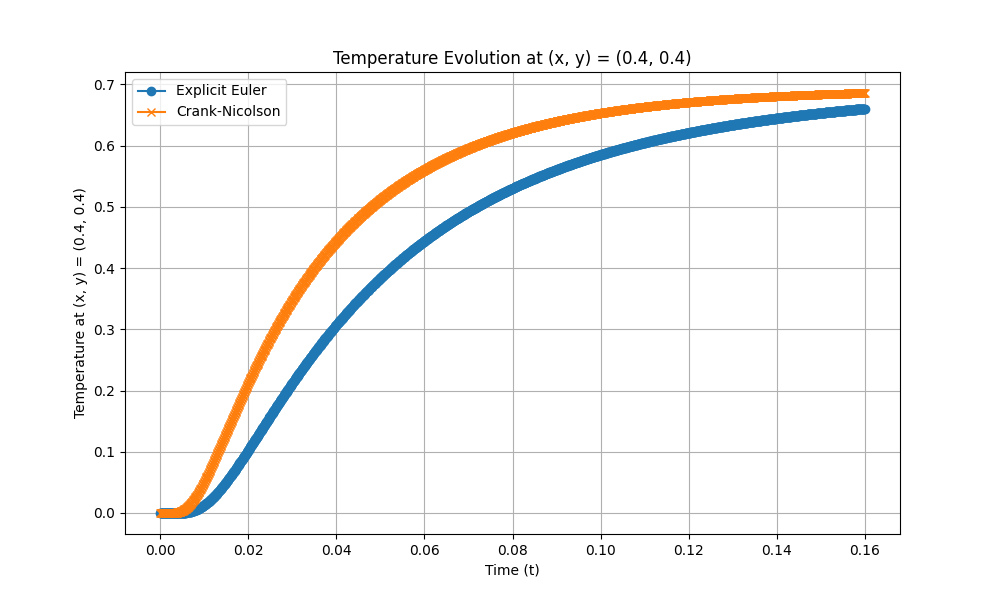
\includegraphics[width=0.5\textwidth]{temperature_evolution_of_a_point_0-0001.png}
\caption{Temperature evolution for point (x, y) = (0.4, 0.4) with $\Delta t = 0.0001$}
\label{fig: point evolution}
\end{figure}

From the picture we can see that both methods show a gradual increase in temperature as time progresses, which is consistent with the expected behavior in heat diffusion problems, where the temperature generally rises and stabilizes as the system approaches a steady state.
Crank-Nicolson solution reaches a higher temperature faster than the Explicit Euler solution, probably because it captures more accurately the diffusion process. 
However both solutions approach a steady state when the time progresses: Explicit Euler reaches this state more gradually, while Crank-Nicolson reaches it earlier indicating faster convergence.

The vertical temperature profile at $t = 0.16$ and $x = 0.4$ can be generated as well using the file plotsgenerator.py, and it is reported below.
\begin{figure}[h]
\centering
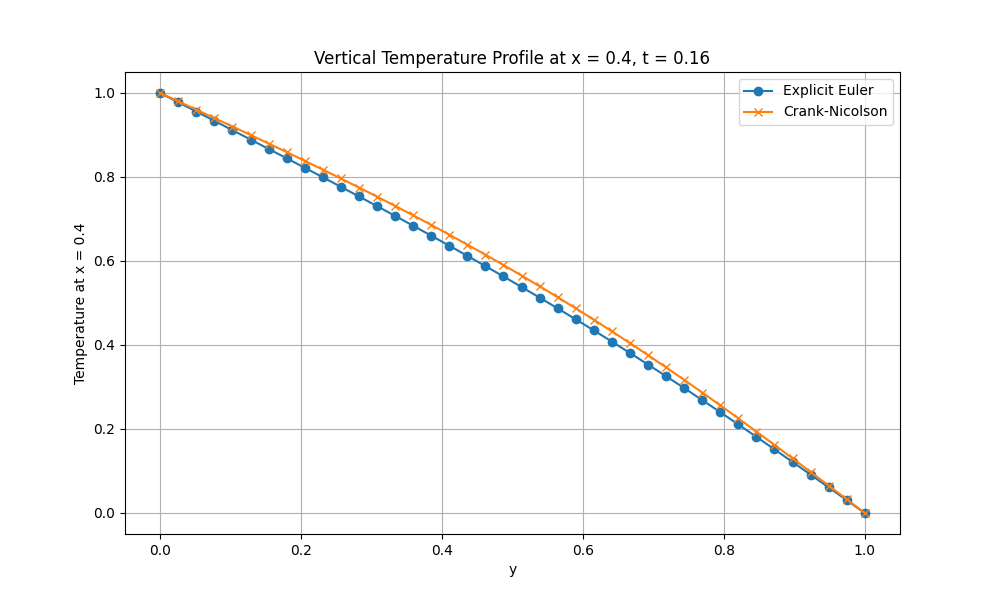
\includegraphics[width=0.5\textwidth]{final_temperature_along_a_line0-0001.png}
\caption{Vertical temperature profile at $t = 0.16$ and $x = 0.4$ with $\Delta t = 0.0001$}
\label{fig: vertical temperature}
\end{figure}

The temperature profile decreases smoothly from $y = 0$ to $y = 1$, indicating a gradient that is consistent with heat diffusion from a higher temperature boundary to a lower one.
Both methods produce very similar results across the entire $y$-axis. This similarity suggests that by time $t = 0.16$ both methods have closely approximated the true temperature distribution, so the differences in the initial evolution of the solution reduce as the solution approaches the steady-state.

In evaluating the performance of the Explicit Euler and Crank-Nicolson methods in the implementation of a CFD solver, several observations can be made. Using a spatial discretization of 
$\Delta x = \Delta y = \frac{1}{40}$ and 1600 time steps, the Explicit Euler method required 0.1449 seconds and the Crank-Nicolson method took 10.9192 seconds.

While the Explicit Euler method demonstrates a significant advantage in computational speed, the Crank-Nicolson method offers higher accuracy, being a second-order method in both time and space. Additionally, a crucial advantage of the Crank-Nicolson scheme is its unconditional stability, which allows it to operate without needing to adjust the time step 
$ \Delta t$ in relation to $\Delta x$. In contrast, the Explicit Euler method requires that $\Delta x^2$ and $\Delta t$ maintain a specific ratio to satisfy the CFL (Courant-Friedrichs-Lewy) condition for stability. This constraint can limit the flexibility and accuracy of the Explicit Euler approach when finer spatial discretizations are needed.


\section*{\Large Task 1.4:}

Yes, there are noticeable differences in the contour plots when changing the spatial resolution and/or the time step.
Using a fixed spatial resolution of \( \Delta x = \Delta y = \frac{1}{40} \) with a number of time steps of 160, we observe that 
the solution becomes unstable because the time step violates the Von Neumann stability criterion for the explicit Euler method.

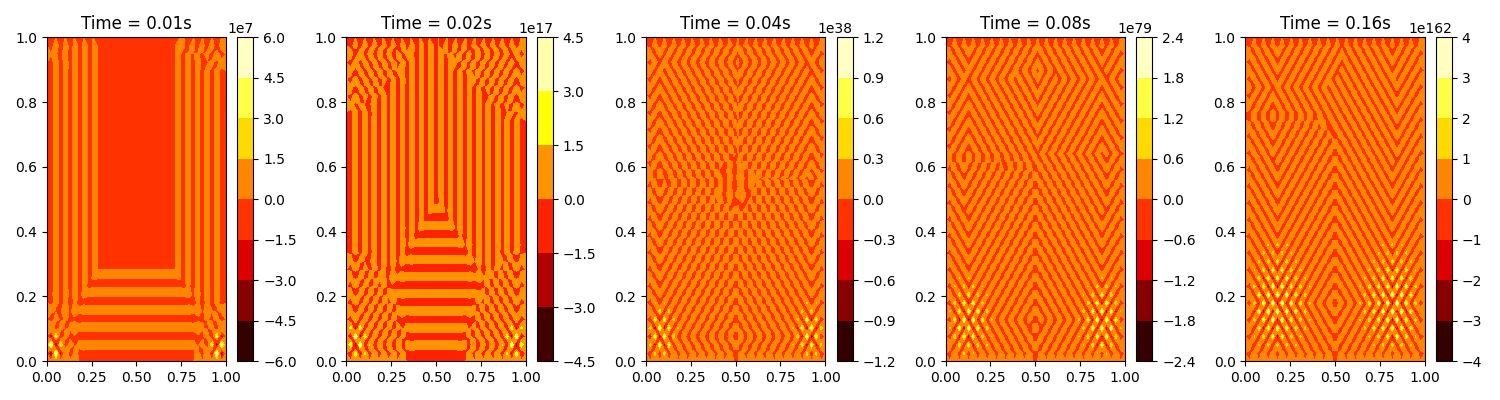
\includegraphics[width=\textwidth]{Figure_1.png}\par\vspace{1cm}

The stability condition ensures that errors introduced at each time step do not grow exponentially as
the computation progresses. In particular, for a 2D heat diffusion problem, this condition can be expressed as:

\[
\Delta t \leq \frac{\Delta x^2}{4}
\]

which implies that the minimum required number of time steps must be at least 1024. 
Infact, using a number of time steps of 1600 the solution becomes stable:

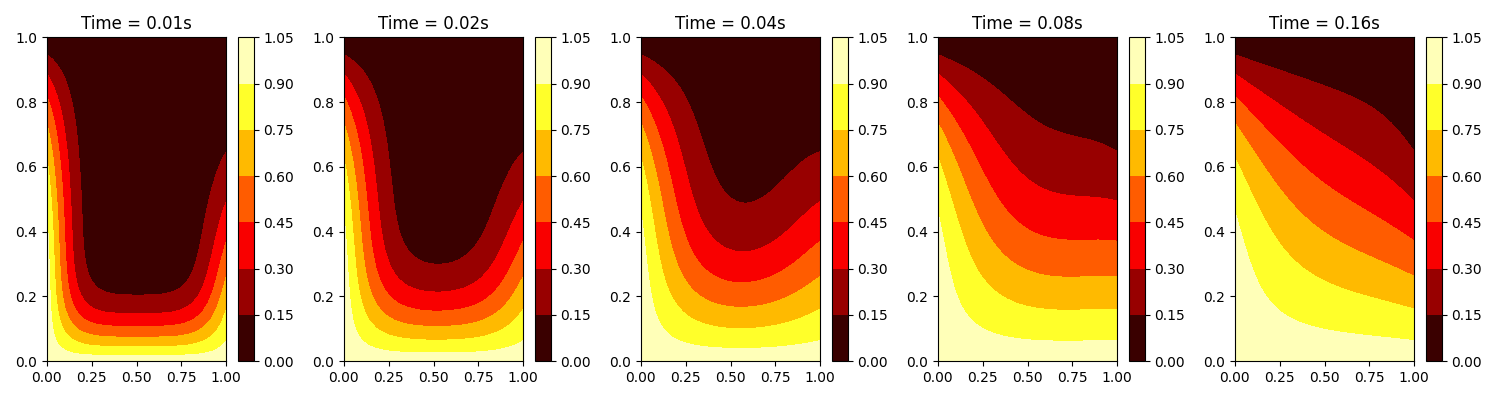
\includegraphics[width=\textwidth]{Figure_2.png}\par\vspace{1cm}

Similarly, using a finer spatial resolution of \( \Delta x = \Delta y = \frac{1}{100} \) with a number of
time steps of 1600 the solution becomes unstable because the minimum number of time steps for stability must be 6400.

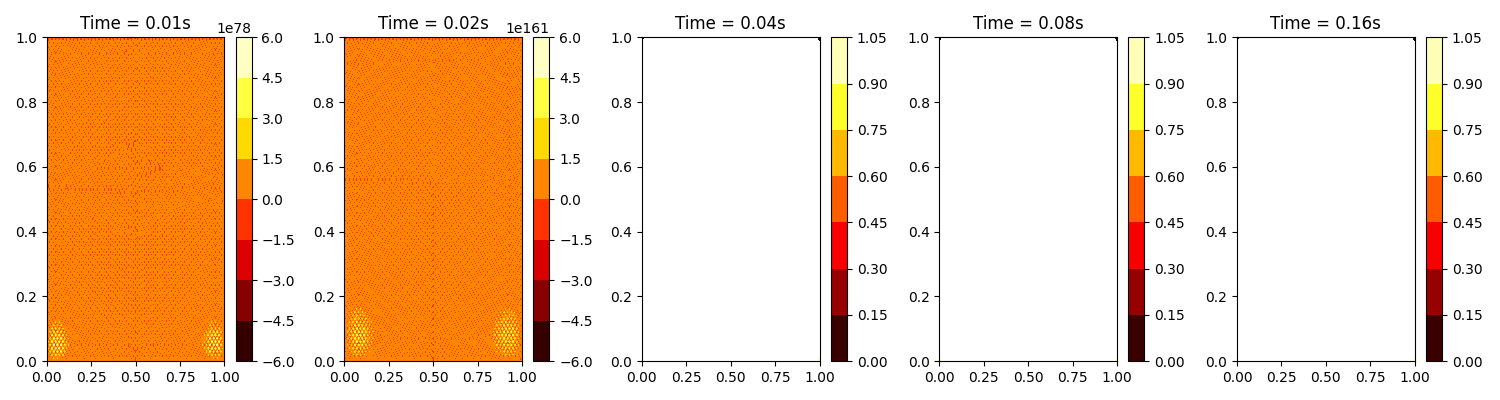
\includegraphics[width=\textwidth]{Figure_3.png}\par\vspace{1cm}

Higher spatial resolution allows for a more accurate representation of temperature but requires smaller
time steps to maintain stability. Infact, with a number of time steps of 6400, the solution becomes stable:

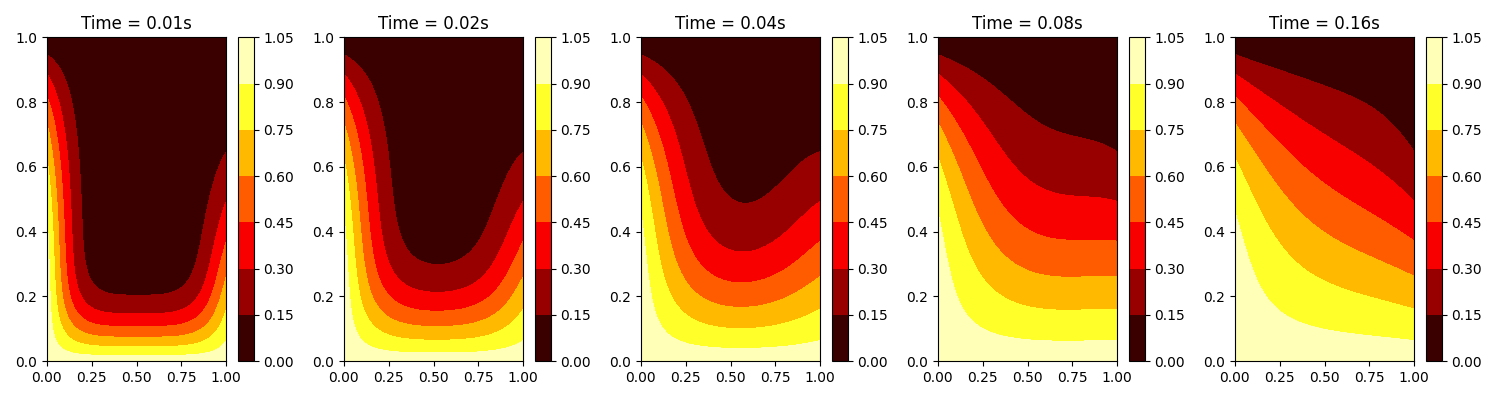
\includegraphics[width=\textwidth]{Figure_4.png}\par\vspace{1cm}

The stability of the solution depends on the ratio between \( \Delta t \) and \( \Delta x \). For finer grids, a smaller \( \Delta t \) 
is required to avoid instability. The choice of time values that are factors of 2 apart \( (t = 0.01, 0.02, 0.04, 0.08, 0.16) \) helps us
understand how heat diffusion evolves over time, allowing us to observe the progression of the temperature field at exponentially increasing 
intervals. Using exponentially increasing time steps provides a clear and efficient view of both the rapid initial diffusion and the slower, 
later stages, without requiring an excessive number of snapshots.


\begin{thebibliography}{9}
    \bibitem{GitHubRepo}
    \textit{CFD Repository},\\
    Available at: \url{https://github.com/GiuseppePisante/CFD.git}
    
    \bibitem{GitHubCopilot}
    \textit{GitHub Copilot},\\
    GitHub. Available at: \url{https://github.com/features/copilot}
    \end{thebibliography}

\end{document}